% Use the following line _only_ if you're still using LaTeX 2.09.
%\documentstyle[icml2012,epsf,natbib]{article}
% If you rely on Latex2e packages, like most moden people use this:
\documentclass{article}

% For figures
\usepackage{graphicx} % more modern
%\usepackage{epsfig} % less modern
\usepackage{subfigure} 

% For citations
\usepackage{natbib}

% For algorithms
\usepackage{algorithm}
\usepackage{algorithmic}

% As of 2011, we use the hyperref package to produce hyperlinks in the
% resulting PDF.  If this breaks your system, please commend out the
% following usepackage line and replace \usepackage{icml2012} with
% \usepackage[nohyperref]{icml2012} above.
\usepackage{hyperref}

% Packages hyperref and algorithmic misbehave sometimes.  We can fix
% this with the following command.
\newcommand{\theHalgorithm}{\arabic{algorithm}}

% Employ the following version of the ``usepackage'' statement for
% submitting the draft version of the paper for review.  This will set
% the note in the first column to ``Under review.  Do not distribute.''
\usepackage{icml2012} 
% Employ this version of the ``usepackage'' statement after the paper has
% been accepted, when creating the final version.  This will set the
% note in the first column to ``Appearing in''
% \usepackage[accepted]{icml2012}


% The \icmltitle you define below is probably too long as a header.
% Therefore, a short form for the running title is supplied here:
\icmltitlerunning{Submission and Formatting Instructions for ICML 2012}

\begin{document} 

\twocolumn[
\icmltitle{CS 4780 Final Project Report}

% You may provide any keywords that you 
% find helpful for describing your paper; these are used to populate 
% the "keywords" metadata in the PDF but will not be shown in the document
\icmlkeywords{boring formatting information, machine learning, ICML}

\vskip 0.3in
]

\section{Introduction}
Our project focused on a Kaggle dataset from DonorsChoose.org, a twelve year old website that allows teachers to raise money for their classroom projects online. Donorschoose differs from from other crowdfunding platforms in that all donations are philanthropic, rather than granting rewards for backers. Additionally, teachers cannot raise money in excess of their goal, but if the goal is not met the teacher does not receive any of the money. By running and analyzing machine learning algorithms on project data provided by DonorsChoose.org, we hope to determine what factors a teacher can alter to maximize their chance of getting funded. 

Our overall approach was to use a combination of supervised machine learning techniques and statistical analysis to derive the factors that have the biggest impact in getting a project funded. In this pursuit, we tried svms with various kernels, decision trees, and random forests to try to learn predictive hypotheses, and then analyzed the structure of these optimal hypotheses. Related work in this area focuses on predicting success after the projects start via trends in social media, comparing money raised at different intervals, and determining the effect of a creator with a strong social media presence. In contrast, our work seeks to determine what teachers can do before the launch of the project to increase their chances of successful funding. 

\section{Problem Definition and Methods} 
\subsection{Task Definition}
Our goal was to determine what teacher-controlled factors are most important (most positively correlated) to getting a project funded. We are hopeful that the results of our research can help guide teachers better on how to create stronger projects for Donorschoose.org and lead to more projects being successfully funded. Specifically, some of the questions we hope to answer are what the optimal time for a teacher to launch a project is, what subject areas should they focus on, and how much money they should ask for. 
\subsection{Algorithms and Methods}
The first algorithm we explored was support vector machines (SVM). The idea with SVMs is that we can represent each instance as a vector and try to find a hyperplane that separates the classes. In addition to linear hyperplanes, we used various kernels to try more complex hyperplanes, including polynomial hyperplanes and radial hyperplanes. SVMlight was our SVM tool of choice, for its flexibility in accommodating many different hyperplane approaches.  
For each different kernel type, we explored and attempted to optimize cost, C value, and use of biased hyperplane. From there we compared the results of different kernels to determine which was the most applicable to our problem.

Next we tried Decision Trees, and by extension Random Forests. A decision tree is a series of rules in the form of a tree. To classify a new instance, beginning at the root node of the tree, a particular attribute is examined, and depending on the result the the instance is passed off to one of the next level nodes. This continues until the instance reaches a terminal node, classifying it as the value of that terminal node. Trees are created using the TDIDT method of recursively creating nodes based on maximizing information gain. Early stopping is the preferred method to prevent overfitting. Different parameters into the TDIDT method include max tree depth and cost factor (similar to the -j parameter in an SVM). 

Random Forests involve the creation of many Decision Trees using the above process. A forest classifies an instance i based on the classification made by a made by a majority of its trees on i. Each tree is created using the same TDIDT algorithm, but notably on a randomly chosen subset of the training data, and only permitting itself to split on a given subset of attributes. By doing this, noise in either outlier instances or unimportant attributes is less likely to impact the final decision of the forest algorithm, allowing the forest to better examine the underlying trends in the data. Each Forest involved an odd number of trees to not have to break ties in an arbitrary fashion. Parameters for random forest creation include number of trees, number of samples (as a percent of the training set) given to each TDIDT running, and percent of attributes each TDIDT running was allowed to use to split. The overfitting parameters of max depth and cost factor were dropped in the Random Forest algorithm, because one of the main strengths of the Random Forest approach of averaging the responses of many decision trees is that individual overfitting to noise becomes much less of an issue.

\section{Experimental (and/or Theoretical) Evaluation} 
\subsection{Methodology}
Our main hope was to learn accurate predictors - rules able to correctly classify both positive and negative instances. This was an important goal because, unlike many other problems, simply identifying positive instances at the cost of many false positives is not optimal. Knowing which projects are unlikely to get funded is equally important as knowing which projects are likely to be funded. To establish statistical significance we ran hypothesis tests and McNemar?s test with the null hypothesis that our algorithm has the same success rate as the naive classification algorithms. We showed that we can reject the null hypotheses in the hypothesis tests and the McNemar?s test and thus proved that our algorithms are both different from and more accurate than the naive algorithms. We also computed 95\% confidence intervals to show the range of the true means of our algorithms.

Support Vector Machines answer this question by their construction of the optimal weight vector w. By examining the value of w used in the optimal SVM hypothesis, we determined the relative weight of different attributes in the data, thereby identifying the most significant attributes. Decision Trees and Random Forests pertain to this goal by the information they contain in their structure. The nodes at the top of the tree (or at the top of a majority of trees for forests) represent the attributes of a project instance that best distinguish funded projects from non-funded projects - they were selected as such by the information gain rule. By learning a statistically significant decision tree or random forest, we could examine the makeup of those trees and make conclusions on their structures, identifying key project attributes.

Because this is a Kaggle project, Kaggle provided the training and testing data. The provided data is actual project and funding data collected from DonorsChoose.org from September 2002 to December 2013. We selected a subset of 100,000 clean instances from the provided data to use, and randomly partitioned that subset into ten approximately 10,000 instance sections for use as training, validating, and testing sets. One of the first issues we ran into is that approximately 70\% of projects on DonorsChoose.org get funded. Thus any learning algorithm must beat the naive approach of classifying all instances as positive (funded), and achieving an accuracy of approximately 70\%. While we did run tests on this data, we also wanted to see how our approaches would fare against an even set of data (50\% positive), so we created sets of even ?fifty-fifty? data by randomly selecting and pairing equal numbers of positive and negative examples for each set of approximately 10,000 instances. Some of the features such as primary subject matter had multiple possible values.  Initially we represented these characteristics as enums. SVMs assume that real-numbered values that are closer together imply similarity, whereas the real numbers we assigned to the different enum values had no sequential significance. This caused the SVM to miss trends among enums when they may have been present. To handle this we created a new set of binarized data, converting all enums to a series of binary attributes for each possible enum value.  

For every algorithm, we ran a full train-validate-test framework. We selected train, validate, and test sets from the ten divided sections. From there, we trained the algorithm with all combinations of arguments on the train set to create a set of hypotheses. Each hypothesis was preliminarily tested on the validation set. The hypothesis with the highest accuracy on the validation set was outputted and tested on the test set to achieve final metrics. From this final test, we collected accuracy, precision, recall, F-1, and a full set of (Actual Label, Classified Label) tuples of instances in the test set. In the results section we examine the effect of different argument lists on the performance metrics to determine if there is any correlation between input and output metrics, what the optimal argument input is for each algorithm, and the makeup of the optimal hypotheses. 

\subsection{Results}
Singleton decision trees did not achieve notable success, producing equivalent results to naively guessing positive (funded) on all instances. Random forests did produce significantly better results, however. The best Random Forest for the binarized data was achieved using full attribute selection (1.0), a 100\% training set usage, and a 201 trees (the odd number was chosen to avoid classification ties), and achieved an accuracy rate of 72.222\%. Using McNemar?s test the number of unique errors for our algorithm and the naive were 353 and 583 respectively. This gives that the probability that these two algorithms come from the same distribution is $2.69*10^{-14}$, so we concluded that these two algorithms are not from the same distribution. Hypothesis testing with a significance level of 99\% shows that the chance we would get 7207/9979 correct classifications given a success rate of $0.6991$ or less is only $1.86*10^{-7}$. Thus we rejected the null hypothesis and concluded that our algorithm does indeed have a success rate greater than the naive classification on the original binarized data. We also calculated that the true success rate of our algorithm is in the range $[.713, .731]$ with 95\% confidence.

From here we ran tests to determine which of the attributes in this best performing Random Forest caused it to outperform its neighbors. Both attribute selection and training set usage were uncorrelated with any of the performance metrics. Number of trees, however, has a strong correlation with performance (accuracy). Accuracy improves when moving from a single tree towards 201 trees, then slides back towards the naive success rate of 69.8\%. (See fig. 1, in appendix).
Random Forests performed even better on the binarized and equalized data, vastly outperforming the naive success rate of 50\% and improving with number of trees.  (See fig. 2, in appendix)

Accuracy, Recall, and F-1 reach a peak at 51 trees, whereas Precision continues to rise until 101 trees. The peak accuracy at 64.55\% was achieved with 51 trees. McNemar?s test similarly showed that the given errors under the same distribution occur with a probability of $2.02*10^{-63}$ so we can conclude that our algorithm is not from the same distribution as the naive algorithm which classifies correctly 50\% of the time. Hypothesis testing at a significance level of 99\% similarly shows that we can achieve such success with probability virtually zero (less than $1*10^{-20}$) given that our true success rate is 50\% or less. Thus we can reject the null hypothesis and conclude that our algorithm does indeed have a success rate greater than the naive classification (50\%) on the 50/50 binarized data.

In our SVM approach, we found biased hyperplanes to perform better than unbiased hyperplanes. Initially the most significant attributes were longitude, latitude, and the amount of money being requested.  We quickly noted that these were the largest values, thus caused the greatest impact within the svm algorithm. We resolved this issue by normalizing attributes across all of the data. For kernels we found that polynomial and radial basis function both worked well, but that linear and sigmoid did not fit the data. Initially when cost was 1, all values were labeled positive, thus the SVM did not learn any better than the naive approach.  We found a cost of 0.75 to work well and explored similar values such as 0.6, 0.7, 0.8. The optimal C value was dependent on the other parameters.  Our strategy was to start with 10, 100, 1000 and then do a few iterations of binary search based on the which of those values performed best. Despite the sheer magnitude of arguments we provided, however, we could not learn a significant rule using SVMlight.  

After breaking down the data and analyzing subsets of the data we were able to find some interesting trends. First, the success rate of funding is correlated with the month of the year that the campaign was started with a cyclic trend. The peak of success is in December with a success rate of 76\% and the lowest rate of success comes in June with a success rate of 61\%. Success in funding increases from June to December and decreases from December to June almost monotonically. These findings are shown in fig 3. (See appendix).

We also found that teachers with more projects tend to do better with each new project they attempt over time, (See fig 4, in appendix), showing that the cumulative success rate of teachers increases as the number of projects they propose increases.

A similar trend with schools was found, to a certain extent. Fig 5 shows that cumulative success rate of a school also improves with more projects funded, but if we look at success rate at each specific time ordered project, we see that the trend for schools is not as clear, whereas Fig 6 shows that there is downward trend in success rate after 37 projects have been proposed. 

\subsection{Discussion}

The best accuracy rate for any svm we were able to achieve in any test set was $0.702$. Hypothesis testing with a significance level of 99\% showed that the chance we would get 6996/9966 correct classifications given a success rate of .699 or less (naive classification success rate) is $0.25$. Thus we cannot reject the null hypothesis, because $0.25>0.01$ and conclude that our algorithm does not necessarily have a success rate greater than the naive classification on the original binarized data. 

We investigated the structure of the size 201 Random Forest that achieved the 72.222\% accuracy rate. See fig 7 for a count of the number of splits at depths 1, 2, and 3 that occur on each attribute.

From the graph, it is clear that the single most defining characteristic is, unsurprisingly, the total price of the project. More investigation into this revealed that more expensive projects are less likely to be funded. The second most important attribute is the month during which the project is posted, affirming that the cyclical time trend discussed above does have predictive power over the funding of a project.

\section{Related Work}
In our background readings we found that many people were doing post-mortem analysis of crowdfunding campaigns and looking for metrics to predict success after the project has already started. Vincent Etter, Matthias Grossglauser, Patrick Thiran (http://goo.gl/gWXrtf) looked into modelling the amount of money as a HMM and using KNN to find past projects at a similar state, tracking social media activity around a specific campaign, and graphing the other projects that the backers participated in. They found that the best way of predicting success at a given interval of time was to train a SVM that pulled from the results of modelling the donations and the social media activity. Professor Mollick (http://goo.gl/Pnyu8) tried to understand crowd funding through an analytical perspective and found that the strength of a person?s social network had a major effect in how successful the project was. 

Our work differs from these papers because we?re focusing on what the creators can do to maximize their chance of getting funded as opposed to predicting success once a project has started. We are also using different mechanics to solve our problem than this related work since we?re using machine learning algorithms to extract insights from the data instead of using the data as a basis for future prediction. We?re confident that this approach will yield more meaningful results to the crowdfunding community since we?ll be able to deliver actionable insights instead of statistical significance.

\section{Future Work}
Although we were able to achieve significant improvements at classifying data from an even distribution of positive and negative examples, our best results run on the original data set do not represent much of an improvement over the naive classification approach. We have already exhausted many variants on decision trees and multiple kernels for SVM so the next logical step is to include more data in our analysis. Perhaps the most significant data we did not include in our learning algorithms is a one paragraph blurb that teachers submit along with project proposals. Running some NLP or sentiment analysis on these paragraphs and including this as an attribute to the data could give a significant improvement on our accuracy.

\section{Conclusion} 
Overall, developing a hypothesis that would classify our data significantly better than a naive classifier proved difficult. After cleaning our dataset we were able to successfully predict if a project would be funded or not with 72.22\% accuracy and are 95\% confident that the actual success rate is in the range 71.3\% to 73.1\%, using the random forest algorithm. Based on those results we were able to conclude that teachers who want to maximize their chance of being funded should ask for as little as money as possible, and launch their project between June and December. We hope these results will encourage other researchers to examine the initial characteristics of crowdfunding projects more closely and hopefully we can find more insights that can help teachers and creators of these projects improve their odds of getting funded. 

\section{Appendix}

Fig 1:\\
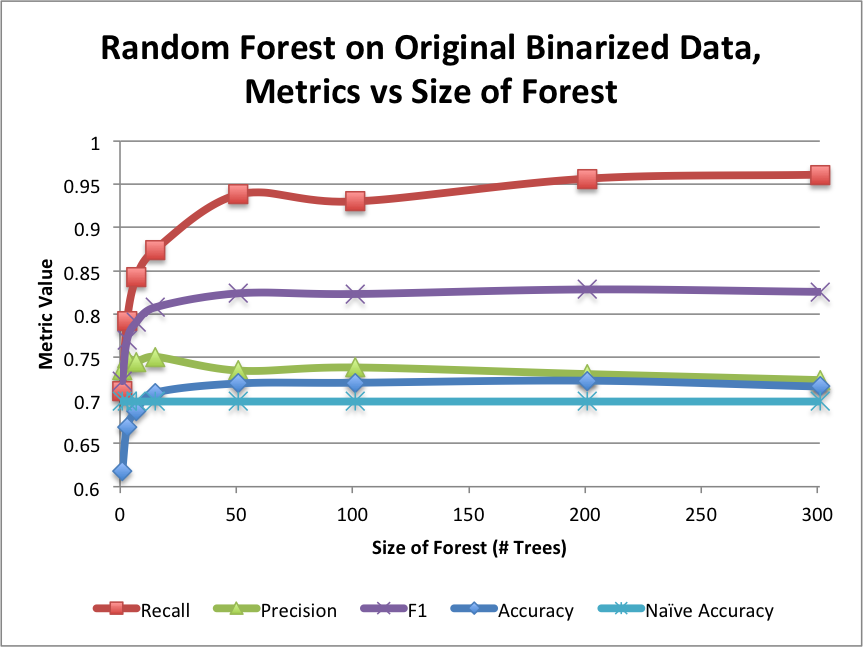
\includegraphics[width=\textwidth / 2]{Forest1.png}
\\\\
Fig 2: \\
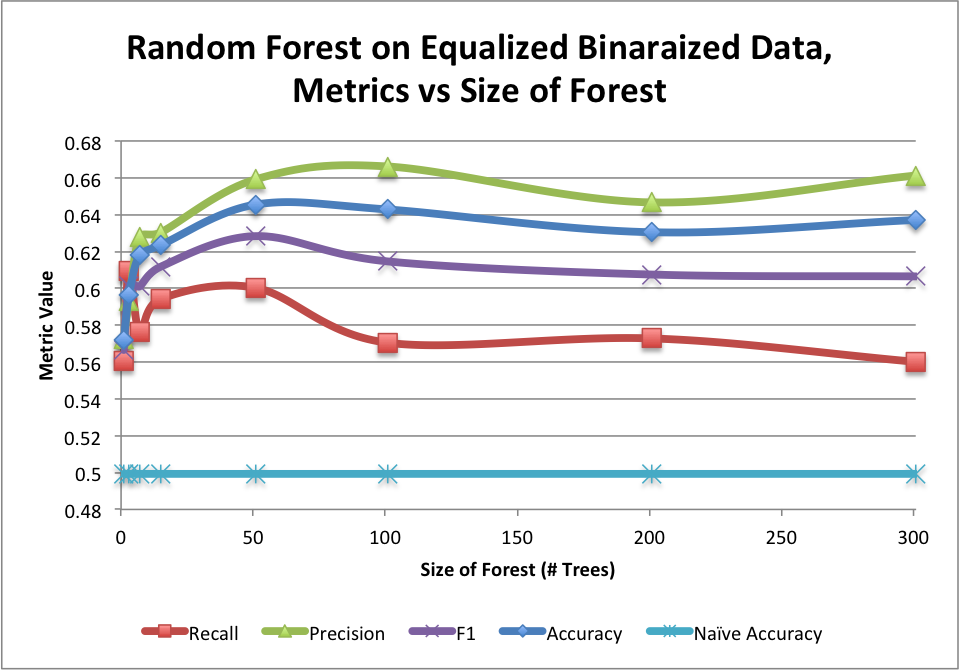
\includegraphics[width=\textwidth / 2]{Forest2.png}
\\\\
Fig 3:\\
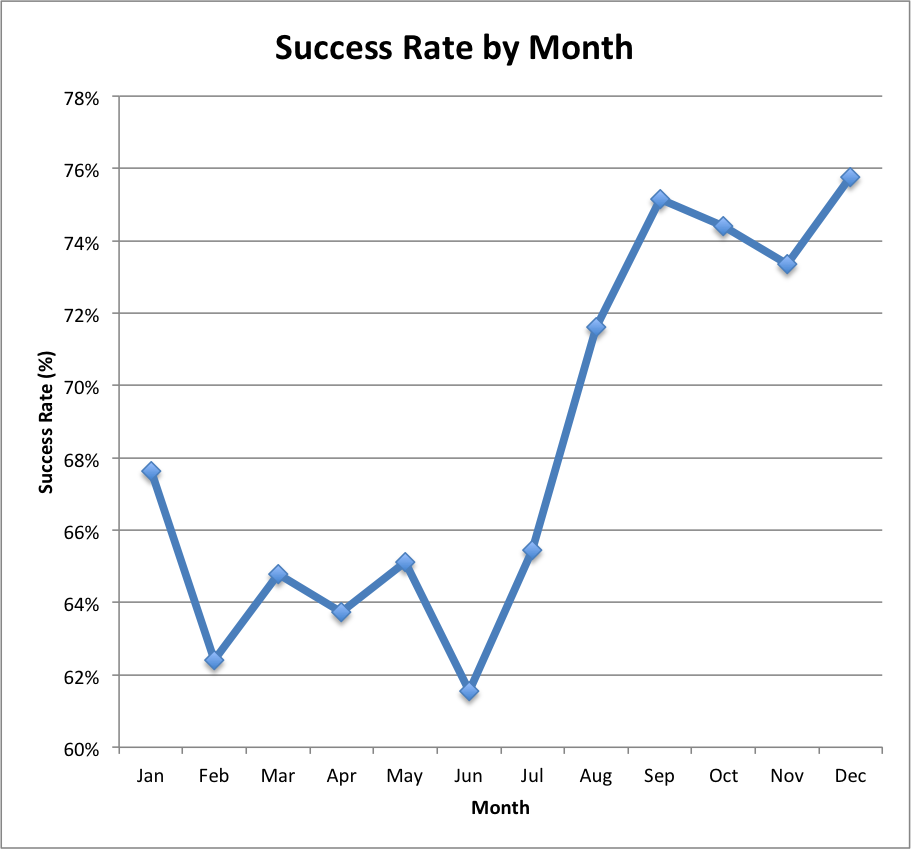
\includegraphics[width=\textwidth / 2]{OverTimeSuccess.png}
\\\\
Fig 4:\\
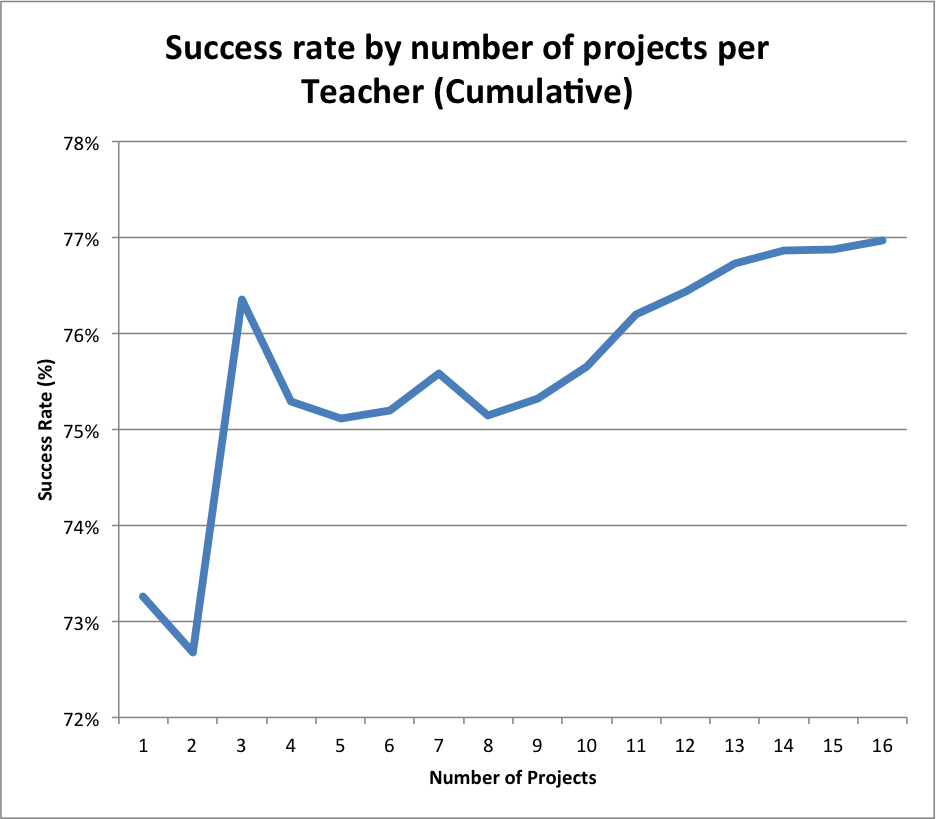
\includegraphics[width=\textwidth / 2]{TeacherSuccess.png}
\\\\
Fig 5:\\
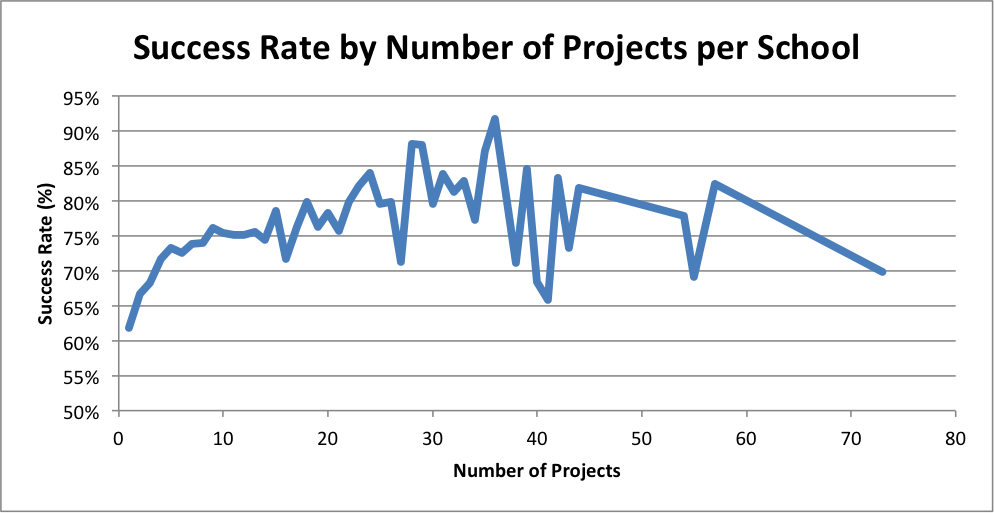
\includegraphics[width=\textwidth / 2]{SchoolSuccess.png}
\\\\
Fig 6:\\
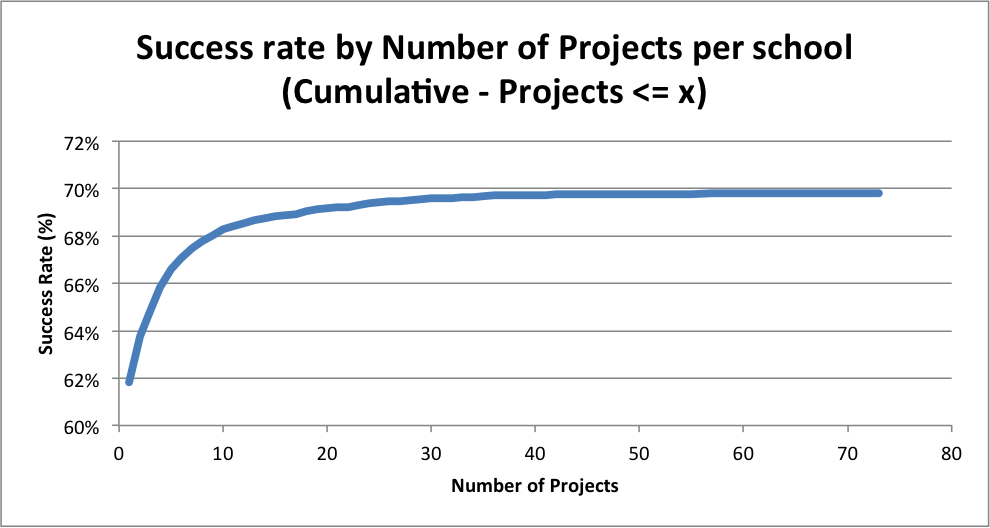
\includegraphics[width=\textwidth / 2]{SchoolSuccessCumulative.png}
\newpage
Fig 7:\\
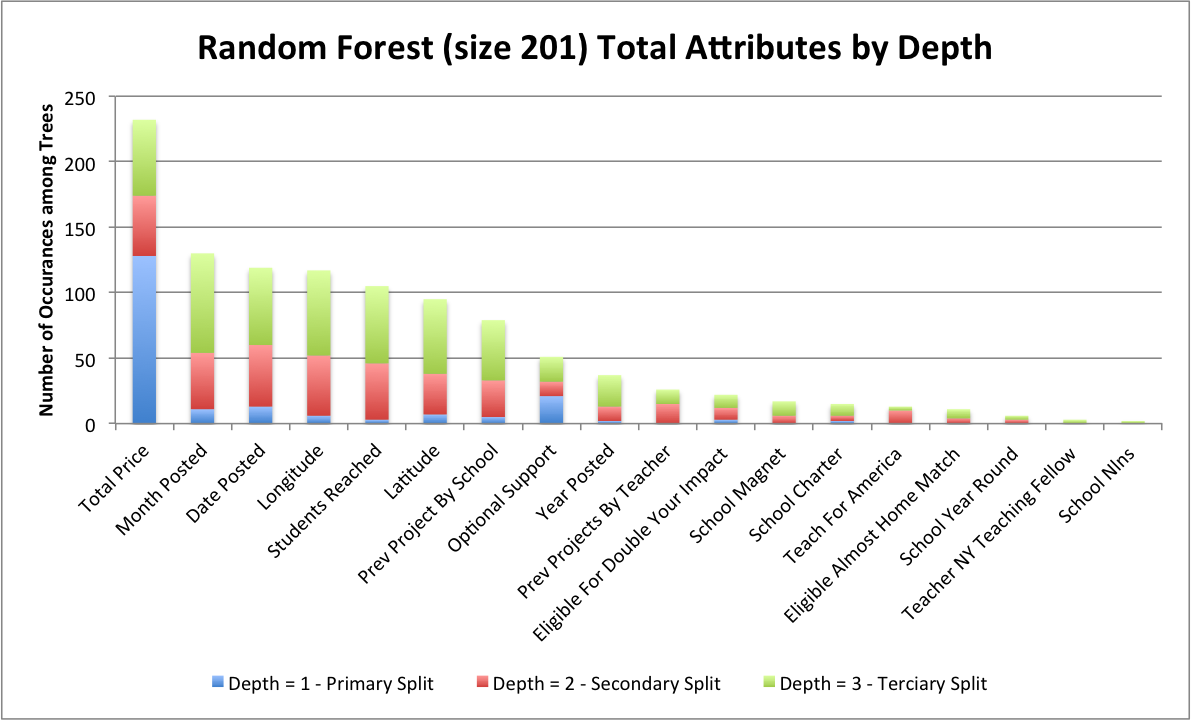
\includegraphics[width=\textwidth]{Forest3.png}

\begin{thebibliography}{3} 
\bibitem{scikit} Fabian Pedregosa, Ga�l Varoquaux, Alexandre Gramfort, Vincent Michel, Bertrand Thirion, Olivier Grisel, Mathieu Blondel, Peter Prettenhofer, Ron Weiss, Vincent Dubourg, Jake Vanderplas, Alexandre Passos, David Cournapeau, Matthieu Brucher, Matthieu Perrot, �douard Duchesnay. \emph{Scikit-learn: Machine Learning in Python}, Journal of Machine Learning Research, 12, 2825-2830 (2011) 
\bibitem{scipy}Jones E, Oliphant E, Peterson P, et al. \emph{SciPy: Open Source Scientific Tools for Python}, 2001-, \url{http://www.scipy.org/} [Online; accessed 2014-12-11].
\bibitem{svm} T. Joachims, Making large-Scale SVM Learning Practical. Advances in Kernel Methods - Support Vector Learning, B. Sch�lkopf and C. Burges and A. Smola (ed.), MIT-Press, 1999. 
\end{thebibliography}

\end{document} 